\documentclass[
  10pt
%, handout
]{beamer}
%\setbeameroption{show notes on second screen}

% TODO: What is this for?
\usepackage{pgfpages}
\usepackage{pdfpages}

% Use T1 Font encoding to support more glyphs
\usepackage[T1]{fontenc}

% Number sections in table of contents
\setbeamertemplate{section in toc}[sections numbered]
% Hide subsections in table of contents
\setcounter{tocdepth}{1}

\usetheme{HPE}

% Also number pages in appendix
\usepackage{appendixnumberbeamer}

% Nicer tables
\usepackage{booktabs}

% foo
\setbeamertemplate{caption}{\raggedright\insertcaption\par}

\usepackage[normalem]{ulem}

\usepackage[scale=2]{ccicons}

\usepackage{pgfplots}
\usepgfplotslibrary{dateplot}

\usepackage{xspace}
\newcommand{\themename}{\textbf{\textsc{metropolis}}\xspace}

\usepackage{graphicx}
\usepackage{listings}

\usepackage{lmodern}

\usepackage{eurosym}
\usepackage{amsmath, amssymb}
\usepackage[binary-units=true]{siunitx}
\DeclareSIUnit{\EUR}{\text{\euro}}

\usepackage{xcolor}
\newcommand\crule[3][black]{\textcolor{#1}{\rule{#2}{#3}}}

\newcommand{\tinycite}[1]{\tiny{(\cite{#1})}}
%\newcommand{\tinycite}[1]{foo}

\title{EDK2 UEFI on RISC-V}
\subtitle{Open Source Firmware, BMC and Bootloader Devroom}
\date{February 6, FOSDEM 2021}
\author{Daniel Schaefer}

\begin{document}

\maketitle

\begin{frame}{Agenda}
  \begin{itemize}
    \item About Us
    \item Introduction (EDK2, RISC-V)
    % To give context
    \item History of Booting on RISC-V
    \item Timeline of This Implementation
    \item Details of Bootflow
    \item Demo Booting to Linux
    \item Status, Goals, Vision
    \item How to Help
  \end{itemize}
  %\tableofcontents
\end{frame}

\begin{frame}{About us}
  \begin{itemize}
    \item UEFI Firmware Engineers for ProLiant Servers at HPE
    \item Learned a lot through this project:\\
          Changes required in entire UEFI/EDK2 boot flow
  \end{itemize}

  \vfill

  \begin{columns}
    \column{0.5\textwidth}
    \begin{figure}[h]
      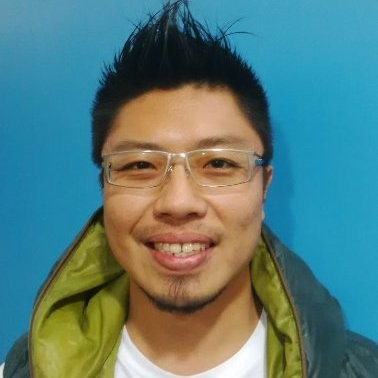
\includegraphics[width=0.3\textwidth]{resources/abner.jpg}
      \caption{Abner Chang}
    \end{figure}
    \begin{itemize}
      \item Senior UEFI Engineer
      \item Lead the project 
    \end{itemize}

    \column{0.5\textwidth}
    \begin{figure}[h]
      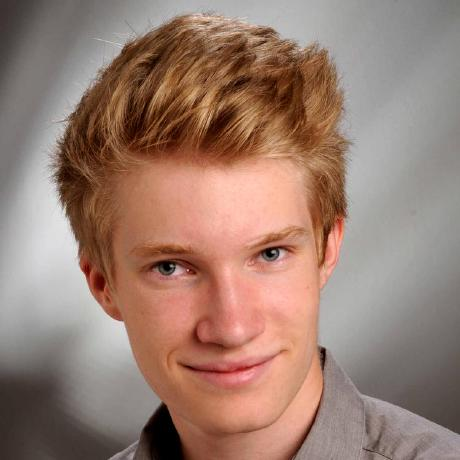
\includegraphics[width=0.3\textwidth]{resources/daniel.jpg}
      \caption{Daniel Schaefer}
    \end{figure}

    \begin{itemize}
      \item Graduated last year
      \item First real UEFI project
    \end{itemize}
  \end{columns}
\end{frame}

\begin{frame}{Disclaimer}
  \begin{itemize}
    \item Work was done on company time
    \item But we can't speak of the strategic direction of HPE
  \end{itemize}
\end{frame}

\begin{frame}{UEFI and EDK2}
  \centering
  
\includegraphics[width=0.3\textwidth]{resources/tianocore-logo.png}

  \vfill

  \begin{itemize}
    \item UEFI is only an interface specification
    \item EDK2 is the reference implementation of UEFI
    \item Initially developed for Itanium 
    \item Now mainstream for x86\_64
    \item Starting to get adopted on ARM % Aarch32 since 2009, Aarch64 since 2013, part of BBR standards...
  \end{itemize}
\end{frame}

\begin{frame}{RISC-V}
  \centering
  
\includegraphics[width=0.3\textwidth]{resources/riscv-logo.png}

  \vfill

  \begin{itemize}
    \item "Free and Open RISC Instruction Set Architecture"
    % Implementations aren't required to be open
    \item Tries to be simple and legacy-free
    \item Three privilege modes (\textbf{M}achine, \textbf{S}upervisor, \textbf{U}ser)
      % Implementations are only required to provide Machine
      % There's now also, optionally, Hypervisor
    \item Similar to x86, boot starts without MMU in Machine mode
      % Firmare and OS have to enable MMU and transition to S&M
    \item FW can stay resident after boot and be called by higher layers \\
          Like x86's SMM but with well defined interface like Itanium's SAL \\
          $\rightarrow$ Supervisor Binary Interface (SBI)
  \end{itemize}
\end{frame}

% TODO: Maybe compare diagrams of SBI and SAL
% TODO: Maybe add a slide of SBI OpenSBI

% We use OpenSBI as an SBI implementation and helper library
% Differently than U-Boot and coreboot we don't use it to load EDK2 or as a payload
% 
% Calling SBI works the same way as userspace makes kernel calls (syscall or ecall in RISC-V)

\begin{frame}{History of booting on RISC-V}
  \begin{tabular}{ll}
    2015 & BBL \\ % Berkeley Boot Loader, original research bootloader
    2016 & EDK2 Prototype with QEMU RISC-V PC/AT board\textsuperscript{\tiny [5]} \\
    2017 & U-Boot \\
    2018 & U-Boot with UEFI interface \\
    2018 & Coreboot \\
    2019 & Oreboot \\ % First version of Oreboot
    2020 & EDK2+OpenSBI Upstream \\
  \end{tabular}
\end{frame}

\begin{frame}{Timeline of this implementation}
  \begin{tabular}{ll}
    2015 & Started at HPE \\
    2016 & Prototype presented at UEFI Forum Plugfest \\
    2020 & Initial upstreaming to EDK2 \\
         & Booting to UEFI shell on Hifive Unleashed \\
    2021 & Upstream Linux EFISTUB support (WIP) \\
    2021 & Port more boards, e.g. BeagleV (WIP) \\
  \end{tabular}
\end{frame}

\begin{frame}{UEFI Phases}
  \begin{center}
    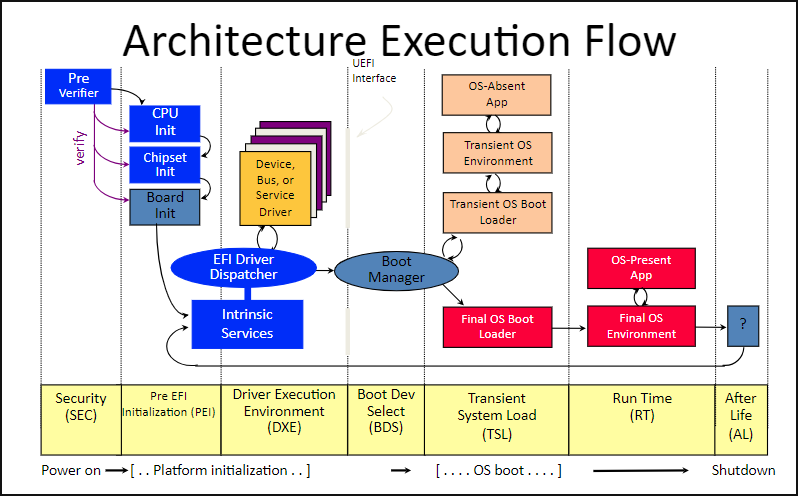
\includegraphics[width=0.8\textwidth]{resources/bootflow.png}
  \end{center}
\end{frame}

\begin{frame}{Reset at ZSBL}
  Walkthrough of Hifive Unleashed Bootflow

  \vfill

  \begin{itemize}
    \item Starts running in M-Mode without MMU
    \item ZSBL (zero stage bootloader)
  \end{itemize}

  \begin{itemize}
    \item Embedded in mask ROM or hardcoded in QEMU source
    \item Jumps to predefined address % We put QEMU there
  \end{itemize}
\end{frame}

\begin{frame}{SEC - First Phase of UEFI (ASM)}
  \begin{itemize}
    \item Fully custom for RISC-V
    \item Starts in assembly % Very easy to write, compared to x86
  \end{itemize}

  \begin{enumerate}
    \item Set up scratch register (mscratch) % Used to pass information to sbi_init
    \item Set up stack in temporary RAM
    \item Set up trap handler to preserve registers and call OpenSBI
    %- Set up trap handler
    %  - Check privilege mode
    %  - Save registers
    %  - Call OpenSBI's trap handler
    %  - Restore registers
    \item Calls SEC core C function with hartid and scratch pointer
  \end{enumerate}

  % Platform/RISC-V/PlatformPkg/Universal/Sec/Riscv64/SecEntry.S
\end{frame}

\begin{frame}{SEC - First Phase of UEFI (C)}
  \begin{enumerate}
    \item Add UEFI private region in scratch space
    \begin{itemize}
      \item Machine information (march, mimpid, ...)
    \end{itemize}
    \item Initialize OpenSBI (sbi\_init)
    \begin{itemize}
      \item Stall non-booting harts
    \end{itemize}
  \end{enumerate}
  % Platform/RISC-V/PlatformPkg/Universal/Sec/SecMain.c
\end{frame}

\begin{frame}{SEC - Initialize OpenSBI}
  \begin{enumerate}
    \item Pass scratch pointer with
    \begin{itemize}
      \item Device Tree % OpenSBI wants to fix it up in sbi_init, not sure if that's still necessary
      \item Next mode (M-Mode still)
      \item Platform specific functions
      %- PLIC, CLIC config
      %- PMP config to make SEC and PEI code rx only, adapted from OpenSBI source file
    \end{itemize}
    \item Register custom SBI calls (avoid linking PEI to OpenSBI)
    %- To get mscratch for current or arbitrary hart
    %- TODO: Should deregister this later because it's only supposed to be used by UEFI
    % I think (Open)SBI doesn't yet have a way to do this
  \end{enumerate}
\end{frame}

\begin{frame}{SEC - Switch to PEI}
  \begin{enumerate} % TODO Start at proper offset
    \item Find PEI entrypoint in firmware volume
    \item Switch to S-Mode
    % Originally we used M-Mode still but it's good to reduce privileges early on and enable MMU
    \item Enable identity mapped MMU
    \item Jump to PEI and pass it information about
    \begin{itemize}
      \item Boot firmware volume
      \item Temporary ram
      \item Stack
    \end{itemize}
  \end{enumerate}
  % Platform/RISC-V/PlatformPkg/Universal/Sec/SecMain.c
\end{frame}

\begin{frame}{PEI}
  From here on most of the code is arch-agnostic in EDK2.
  \vfill
  \begin{enumerate}
    \item Discover RAM and migrate there
    \item Dispatch PEIMs
      \begin{itemize}
        \item Take device tree from scratch space and store in HOB
        \item Discover processor features and store in HOB (For SMBIOS)
        \item Others ...
      \end{itemize}
    % Start DXE
    \item Build new stack
    \item Switch stack and execute DxeIpl
    % Previously this was where we switched to S-Mode and initialize OpenSBI
    % But we want to initialize OpenSBI earlier and have less privileges earlier
  \end{enumerate}
\end{frame}

\begin{frame}{DXE - Dispatch DXEs}
  \begin{itemize}
    \item Install timer interrupt handler and DXE Protocol
    \item Install RuntimeServices (WIP)
    \item Install SMBIOS tables using information from PEI
      \begin{itemize}
        \item Type 4 (CPU)
        \item Type 7 (Caches)
        \item \textbf{Type 44} (Additional CPU information)
      \end{itemize}
    \item Install device tree
      \begin{itemize}
        \item Extract from HOB
        \item Insert boot hartid (required by Linux)
        \item Insert into EFI System Configuration Table
      \end{itemize}
  \end{itemize}
  % https://github.com/riscv/riscv-smbios/
\end{frame}

\begin{frame}{BDS - UEFI Shell}
  Not upstream yet. \\
  Prep: Embed EFISTUB and initrd disk image in flash image

  \vfill

  \begin{enumerate}
    \item Load disk into memory and turn into ramdisk with shell command
    \item Install initrd on handle of fixed device path (`initrd`)
    \item Execute EFISTUB
  \end{enumerate}
\end{frame}

\begin{frame}{EFISTUB - Since Linux 5.10}
  Implemented by Atish Patra, tested and finalized in cooperation with us

  \vfill

  \begin{enumerate}
    \item Take device tree from EFI System Configuration Table
    \item Call LoadFile2 on device path to extract initrd
    \item Execute kernel proper
    \begin{itemize}
      \item Disable MMU
      \item jump\_kernel(hartid, fdt);
    \end{itemize}
  \end{enumerate}
\end{frame}

\begin{frame}{RISC-V EDK2 Phases}
    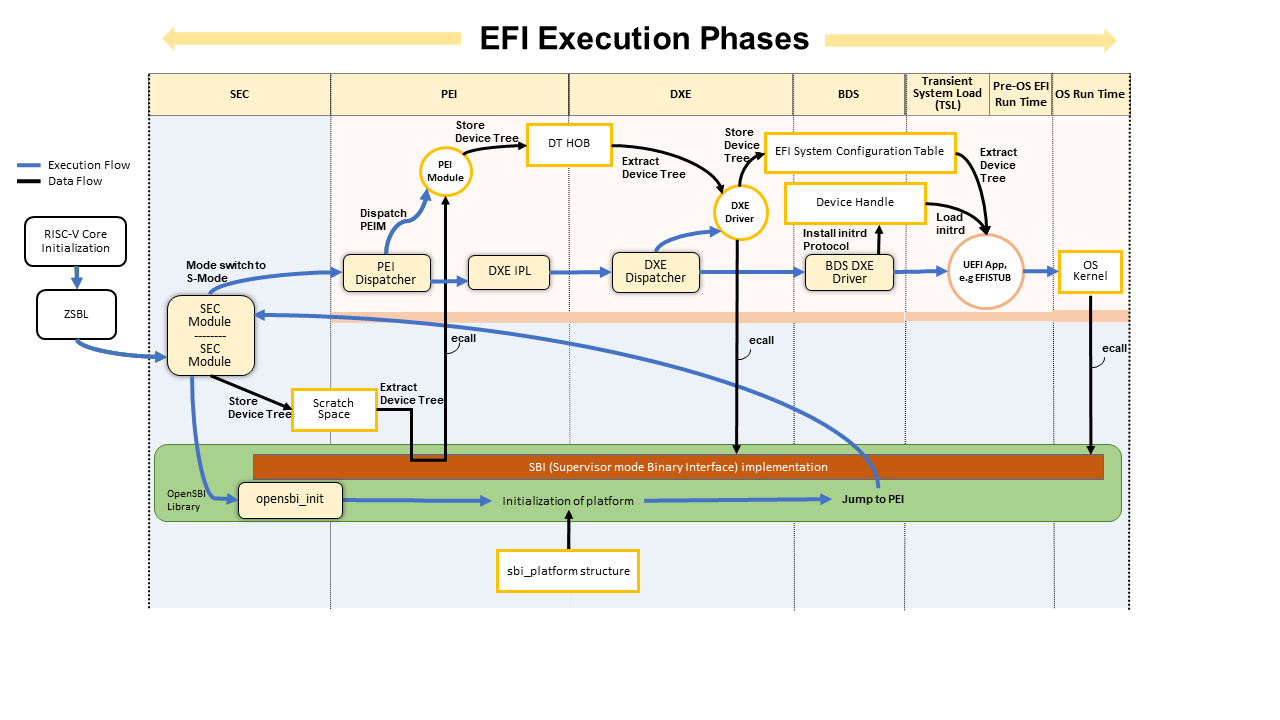
\includegraphics[width=1.15\textwidth]{resources/bootflow-annotated.png}
\end{frame}

\begin{frame}{Demo Booting to Linux}
  \begin{center}
     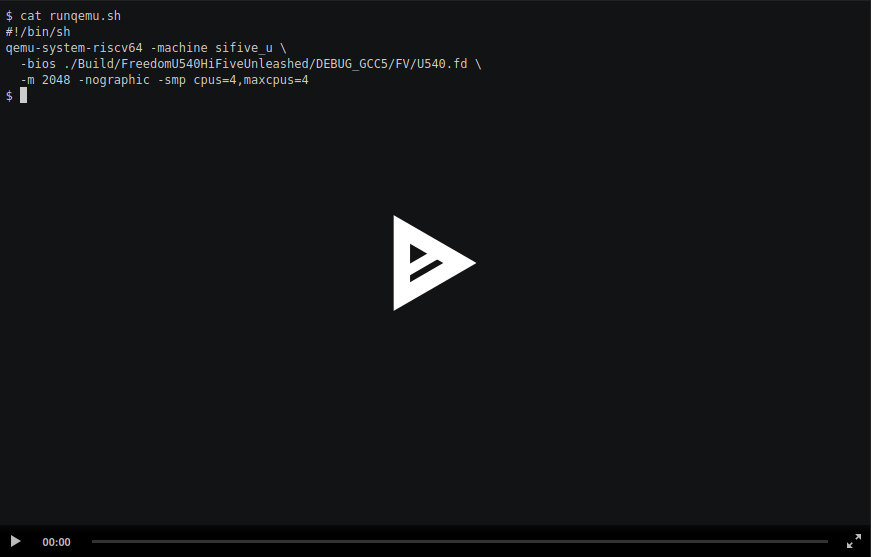
\includegraphics[width=0.75\textwidth]{resources/asciinema.png}
    \href{https://asciinema.org/a/KPDSvhXNVTbsQ45oRUVEu81nY}{https://asciinema.org/a/KPDSvhXNVTbsQ45oRUVEu81nY}
  \end{center}

  \tiny{Firmware image at \href{https://github.com/riscv/riscv-uefi-edk2-docs/releases}{https://github.com/riscv/riscv-uefi-edk2-docs/releases}}

\end{frame}

% TODO: Use proper checkmark and x symbol
\begin{frame}{Status - EDK2}
  \begin{itemize}
    \item UEFI Shell
    \item UEFI Applications (e.g. bootloader)
    \item Booting Linux via EFISTUB
  \end{itemize}
\end{frame}

\begin{frame}{Status - Platforms}
  \begin{center}
    \begin{tabular}{|l|l|l|l|}
      \hline
      Platform Name     & UEFI Shell & Linux \\
      \hline
      HiFive Unleashed  & Yes        & Yes \\
      QEMU sifive\_u    & Yes        & Yes \\
      % VC707
      Freedom U500 FPGA & Yes        & N/A \\
      % Very important! Will help us get proper disk and 
      QEMU virt         & N/A        & N/A \\
      % We have the board, just haven't gotten around to porting it yet
      Andes AE350       & N/A        & N/A \\
      % Registered for early dev board to port until general availability
      BeagleV           & N/A        & N/A \\
      \hline
    \end{tabular}
    % See our status page
  \end{center}
\end{frame}

\begin{frame}{Status - Overall}
  \begin{itemize}
    \item UEFI specification amended
    \item SMBIOS specification amended
    \item EDK2 port merged upstream
    \item Linux EFISTUB ported by Atish, merged in 5.10
    % Haven't tested it on EDK2 yet, but works on U-Boot
    \item UEFI Self Certification Test ported, patches need cleanup
  \end{itemize}
\end{frame}

\begin{frame}{Goals}
  \begin{itemize}
    % OpenSBI 0.9 has support for that
    \item Implement \textit{ResetSystem} Runtime Service with SBI (WIP)\textsuperscript{\tiny [1]}
    \item Upstream changes for booting Linux (FDT fixup and storing)
    \item SD card driver for Hifive Unleashed
    \item Implement new relocation types by newer GNU toolchains\textsuperscript{\tiny [2]}
    \item Build "OVMF" for QEMU's virt platform with VirtIO drivers\textsuperscript{\tiny [3]} \\
          $\rightarrow$ Add boot tests to EDK2 CI \\
          $\rightarrow$ Boot with actual disk! \\
    \item Port to BeagleV when it arrives\textsuperscript{\tiny [4]}
    \item SecureBoot?
  \end{itemize}
\end{frame}

\begin{frame}{How to Help}
  \begin{itemize}
    % - Need to adjust platform
    % - Check what drivers are needed
    % - Create FDF
    \item Port to more boards, talk to us
    \item Check out the issues on the repo
    \item Spread the word
  \end{itemize}
\end{frame}

\begin{frame}{Vision for the Future}
  \begin{itemize}
    \item Make RISC-V boot like rest of industry \\
          U-boot for embedded, UEFI for consumer and server
          % TODO: Not sure about coreboot and LinuxBoot
    \item Follow in ARM's footsteps to \textit{make booting boring}
          % Perhaps we need something like SBBR, EBBR, ...
    \item Encourage discussion about desktops and servers
          % Some companies have started developing powerful chips
  \end{itemize}
\end{frame}

\begin{frame}{Thanks}
  \begin{center}
    \textbf{Thanks for listening!}
  \end{center}

  \vfill

  Check us out on GitHub: \\

  \begin{tabular}{ll}
    Development & Upstream \\
    \hline
    \href{https://github.com/riscv/riscv-uefi-edk2-docs}{riscv/riscv-uefi-edk2-docs} \\
    \href{https://github.com/riscv/riscv-edk2}{riscv/riscv-edk2} & \href{https://github.com/tianocore/edk2}{tianocore/edk2} \\
    \href{https://github.com/riscv/riscv-edk2-platforms}{riscv/edk2-platforms} & \href{https://github.com/tianocore/edk2-platforms}{tianocore/edk2-platforms} \\
  \end{tabular}

  \vfill

  \begin{tabular}{ll}
    Daniel Schaefer & <daniel.schaefer@hpe.com> \\
    Abner Chang     & <abner.chang@hpe.com> \\
  \end{tabular}
\end{frame}

% TODO:
% - https://fosdem.org/2021/schedule/event/firmware_uor/
% - Upload slides

\begin{frame}{References}
  \begin{table}
    \small
    \begin{tabular}{ll}
      UEFI and PI Spec      & \tiny{https://www.uefi.org/specifications} \\
      SBI Spec              & \tiny{https://github.com/riscv/riscv-sbi-doc} \\
      & \\
      {[1]} SBI SystemReset & \tiny{https://github.com/riscv/riscv-sbi-doc/commit/2f101582210b17a6} \\
      {[2]} GOT relocation  & \tiny{https://github.com/riscv/riscv-edk2/issues/3} \\
      {[3]} RISC-V OVMF     & \tiny{https://github.com/riscv/riscv-edk2/issues/2} \\
      {[4]} BeagleV         & \tiny{https://beagleboard.org/beaglev} \\
      {[5]} EDK2 RISC-V in 2016 & \tiny{https://www.youtube.com/watch?v=9c73WHduovs} \\
      & \\
      BBL                   & \tiny{https://www.lowrisc.org/docs/build-berkeley-boot-loader/} \\
      OpenSBI               & \tiny{https://github.com/riscv/opensbi} \\
      U-Boot                & \tiny{https://www.denx.de/wiki/U-Boot} \\
      Coreboot              & \tiny{https://coreboot.org/} \\
      Oreboot               & \tiny{https://github.com/oreboot/oreboot} \\
      QEMU                  & \tiny{https://www.qemu.org/} \\
      Itanium SAL/PAL       & \tiny{https://www.csee.umbc.edu/portal/help/architecture/24535901.pdf} \\
    \end{tabular}
  \end{table}
\end{frame}

\begin{frame}{Glossary}
  \begin{tabular}{ll}
    UEFI      & Unified Extensible Firmware Interface \\
    EDK2      & UEFI's reference implementation \\
    Tianocore & Umbrella name of EDK2 and related projects \\
    MMU       & Memory Management Unit \\
    SBI       & RISC-V interface between S and M-mode \\
    Itanium   & First 64 bit processor by Intel \\
    SAL       & Itanium's System Abstraction Layer \\
    RISC      & Reduced Instruction Set Comuter (vs CISC)\\
    SMM       & System Management Mode \\
    HPE       & Hewlett Packard Enterprise \\
  \end{tabular}
\end{frame}

\end{document}
